\documentclass[class=article, crop=false]{standalone}
%\usepackage[subpreambles=true]{standalone}
\usepackage{import}
%%\usepackage{booktabs}
%\usepackage{tikz}

%\usepackage[utf8]{inputenc}
\usepackage[subpreambles=true]{standalone}
\usepackage{import}
\usepackage{pgfplots}
\pgfplotsset{compat=newest}
\usepgfplotslibrary{groupplots}
\usepgfplotslibrary{dateplot}
\usepackage{caption}
\usepackage{subcaption}
\usepackage{graphicx}
\usepackage{amsmath}
\usepackage{amssymb}
\usepackage[parfill]{parskip}
\usepackage{float}

% \usepackage{pgfplots}
% \usetikzlibrary{pgfplots.groupplots}
% \pgfplotsset{compat=1.9,height=0.3\textheight,legend cell align=left,tick scale binop=\times}
% \pgfplotsset{grid style={loosely dotted,color=darkgray!30!gray,line width=0.6pt},tick style={black,thin}}
% \pgfplotsset{every axis plot/.append style={line width=0.8pt}}
%
% \usepgfplotslibrary{external}
% % Für die Verwendung von 'external' müssen die folgenden Anpassungen in Abhängigkeit der
% % LaTeX Distribution durchgeführt werden:
%
% % fuer Texlive: pdflatex.exe -shell-escape -synctex=1 -interaction=nonstopmode %.tex
% \tikzexternalize[shell escape=-shell-escape]   % fuer TeXLive
%
% % fuer MikTeX:  pdflatex.exe -enable-write18 -synctex=1 -interaction=nonstopmode %.tex
% %\tikzexternalize[shell escape=-enable-write18] % fuer MikTex
%
%
%
% \tikzsetexternalprefix{graphics/pgfplots/} % Ordner muss ev. zuerst haendisch erstellt werden

\begin{document}
\pgfplotsset{width=14cm,compat=1.9}
\section{Octagon}\label{sec:octagon}

We set up an experiment where we can observe drifts and test the accuracy of our system. We taped down 8 straight equidistant lines with 1.5m distance from the middle and marked the 1.5 meter mark on the tape. This way if we drive our robot from point to point, the path will be an octagonal shape where we can see drifts in accuracy over longer periods if we do multiple loops through the same path. We can see a part of this setup in Figure \ref{fig:octagonexp}.

\begin{figure}[H]
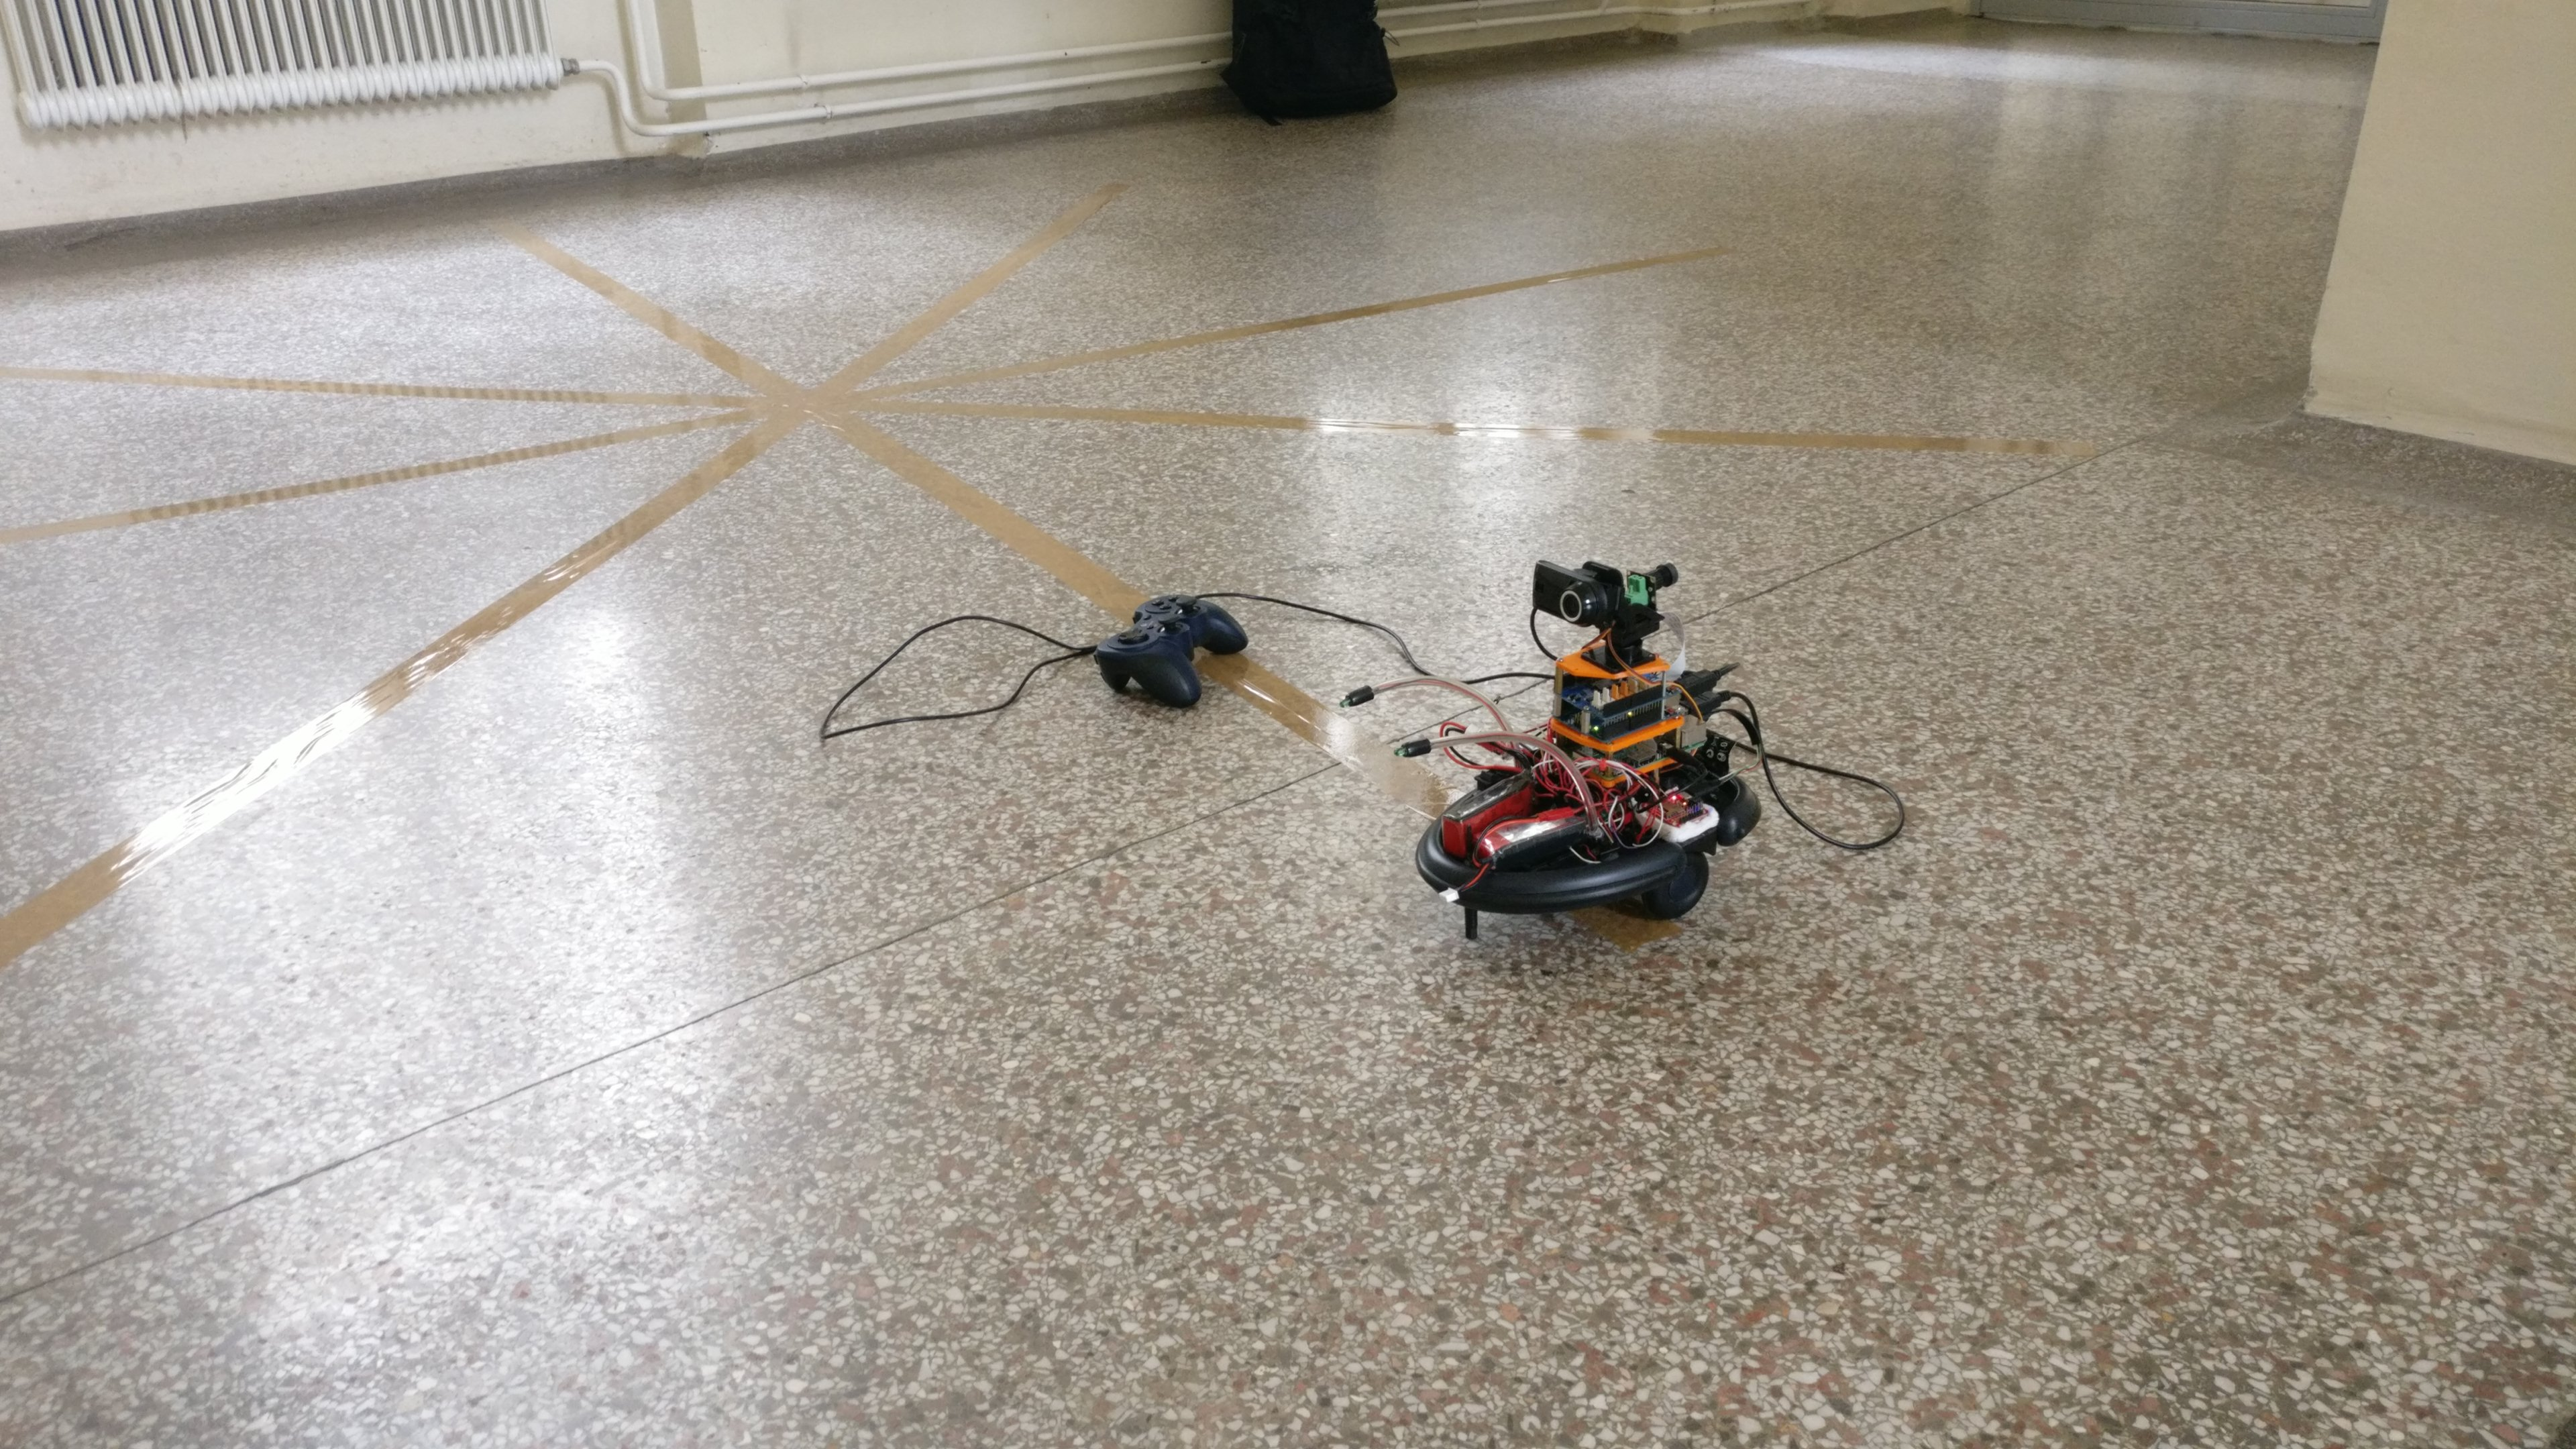
\includegraphics[width=12cm, height=7cm]{images/octagon.jpg}
\caption{Octagon experiment setup}
\end{figure}\label{fig:octagonexp}

\vspace{0.5cm}

We will run the recorded data with our adaptive Kalman Filter and Extended Kalman Filter(EKF) and compare if there are any differences. We used the parameters we set in the section \ref{sec:floor}.

\vspace{0.5cm}

\begin{center}
\begin{figure}[H]
 \begin{flushleft}
  \begin{tikzpicture}
   \begin{axis}[
     yticklabel style={
       /pgf/number format/fixed,
       /pgf/number format/precision=5
      },
     width=12cm,
     height=12cm,
     xlabel={x state [m]},
     ylabel={y state [m]},
     xtick distance= 0.5,
     ytick distance=0.5,
     legend pos=north west,
     grid=both,
     grid style={
       line width=.1pt,
       draw=gray!10},
     major grid style={
       line width=.2pt,
       draw=gray!50
      },
    ]
    \addplot+[color=red, mark=none,line width=1pt,mark size=1pt, dashed] table {plots/octagon_adapt_0_x0x1.csv};
    \addlegendentry{adaptive}
    \addplot+[color=blue, mark=none,line width=1pt,mark size=1pt] table {plots/octagon_ekf_0_x0x1.csv};
    \addlegendentry{EKF}
   \end{axis}
  \end{tikzpicture}
 \end{flushleft}
 \caption{Octagon experiment trajectory comparison}\label{fig:octagonxy}
\end{figure}
\end{center}

\vspace{0.5cm}

\begin{center}
\begin{figure}[H]
 \begin{flushleft}
  \begin{tikzpicture}
   \begin{axis}[
     yticklabel style={
       /pgf/number format/fixed,
       /pgf/number format/precision=5
      },
     width=12cm,
     height=5cm,
     xmax=550,
     domain=0:550,
     ytick distance = 0.5,
     xlabel={Time $[s]$},
     ylabel={x state [m]},
     legend pos=north west,
     grid=both,
     grid style={
       line width=.1pt,
       draw=gray!10},
     major grid style={
       line width=.2pt,
       draw=gray!50
      },
    ]
    \addplot+[color=red, mark=none,line width=1pt,mark size=1pt, dashed] table {plots/octagon_adapt_0_x0.csv};
    \addlegendentry{adaptive}
    \addplot+[color=blue, mark=none,line width=1pt,mark size=1pt] table {plots/octagon_ekf_0_x0.csv};
    \addlegendentry{EKF}
    \addplot+[color=gray, mark=none,line width=1pt,mark size=1pt, samples=2, dashed] {0.0};
   \end{axis}
  \end{tikzpicture}
 \end{flushleft}
 \begin{flushleft}
  \begin{tikzpicture}
   \begin{axis}[
     yticklabel style={
       /pgf/number format/fixed,
       /pgf/number format/precision=5
      },
     width=12cm,
     height=5cm,
     xmax=550,
     ytick distance = 0.5,
     domain=0:550,
     xlabel={Time $[s]$},
     ylabel={y state [m]},
     legend pos=north west,
     grid=both,
     grid style={
       line width=.1pt,
       draw=gray!10},
     major grid style={
       line width=.2pt,
       draw=gray!50
      },
    ]
    \addplot+[color=red,dashed, mark=none,line width=1pt,mark size=1pt] table {plots/octagon_adapt_0_x1.csv};
    \addlegendentry{adaptive}
    \addplot+[color=blue, mark=none,line width=1pt,mark size=1pt] table {plots/octagon_ekf_0_x1.csv};
    \addlegendentry{EKF}
    \addplot+[color=gray, mark=none,line width=1pt,mark size=1pt, samples=2, dashed] {0.0};
   \end{axis}
  \end{tikzpicture}
 \end{flushleft}
\begin{flushleft}
  \begin{tikzpicture}
   \begin{axis}[
     yticklabel style={
       /pgf/number format/fixed,
       /pgf/number format/precision=5
      },
     width=12cm,
     height=5cm,
     ytick distance=1,
     xmax = 550,
     xlabel={Time $[s]$},
     ylabel={$\Psi$ state [rad]},
     legend pos=north west,
     grid=both,
     grid style={
       line width=.1pt,
       draw=gray!10},
     major grid style={
       line width=.2pt,
       draw=gray!50
      },
    ]
    \addplot+[color=red, mark=none,line width=1pt,mark size=1pt, dashed] table {plots/octagon_adapt_0_x3.csv};
    \addlegendentry{adaptive}
    \addplot+[color=blue, mark=none,line width=1pt,mark size=1pt] table {plots/octagon_ekf_0_x3.csv};
    \addlegendentry{EKF}
   \end{axis}
  \end{tikzpicture}
 \end{flushleft}
 \caption{Octagon experiment states}\label{fig:octagon}
\end{figure}
\end{center}

\vspace{0.5cm}

The robot wasn't driven perfectly due to diffulties in turning accurately, but we can observe drifts in both axes and slightly different $\Psi$ states in Figure \ref{fig:octagon}.

The small drifts between the two filters were also observed in the Subsection \ref{subsec:betatesting} and the experiment confirms that EKF can handle the non-linearities in our turns better and give a more reliable $\Psi$ state estimate given a good enough $\varrho^{\eta\chi}$.

\end{document}
